% !TeX root = ../../main.tex

\subsection{Transferring from Gym to Unity 2-DOF Base Environment}

In this experiment, we create a similar environment in Unity to test the transferability between different two physics engine. This experiment is conducted to test the trained agent on a new different environment which has the same observation and action spaces like the environment that was used for training with a different reward function. In this way, we will be using the trained agent from the third experiment to test it on this experiment and observe the performance and behaviour of the agent.

\subsubsection{Setup and configurations}

In this section we describe the setup of the experiment and how it was performed. Firstly, we introduce and describe the RoboReacher robotics arm environment provided by OpenAI Gym and PyBullet physics simulator. Then, based on the environment description, we present the observation space, action space and reward function of the experiment as a base towards the learning process and achieving environment goal. Subsequently, we describe the learning process. For this, we present the reinforcement learning algorithm and neural network architecture used.


\subsubsection{Environment Description}
Using Unity physics engine and Unity ML-Agent, we have built a new 2-DOF robotic environment, shown in the figure below~\ref{fig:unity_reacher}, which is similar to OpenAI Gym environment. The environment has the same observation and action spaces like gym environment and we have modified the reward function to be more complex in this environment to test the behavior of the trained agent.

\begin{figure}[!htb]
		\centering
				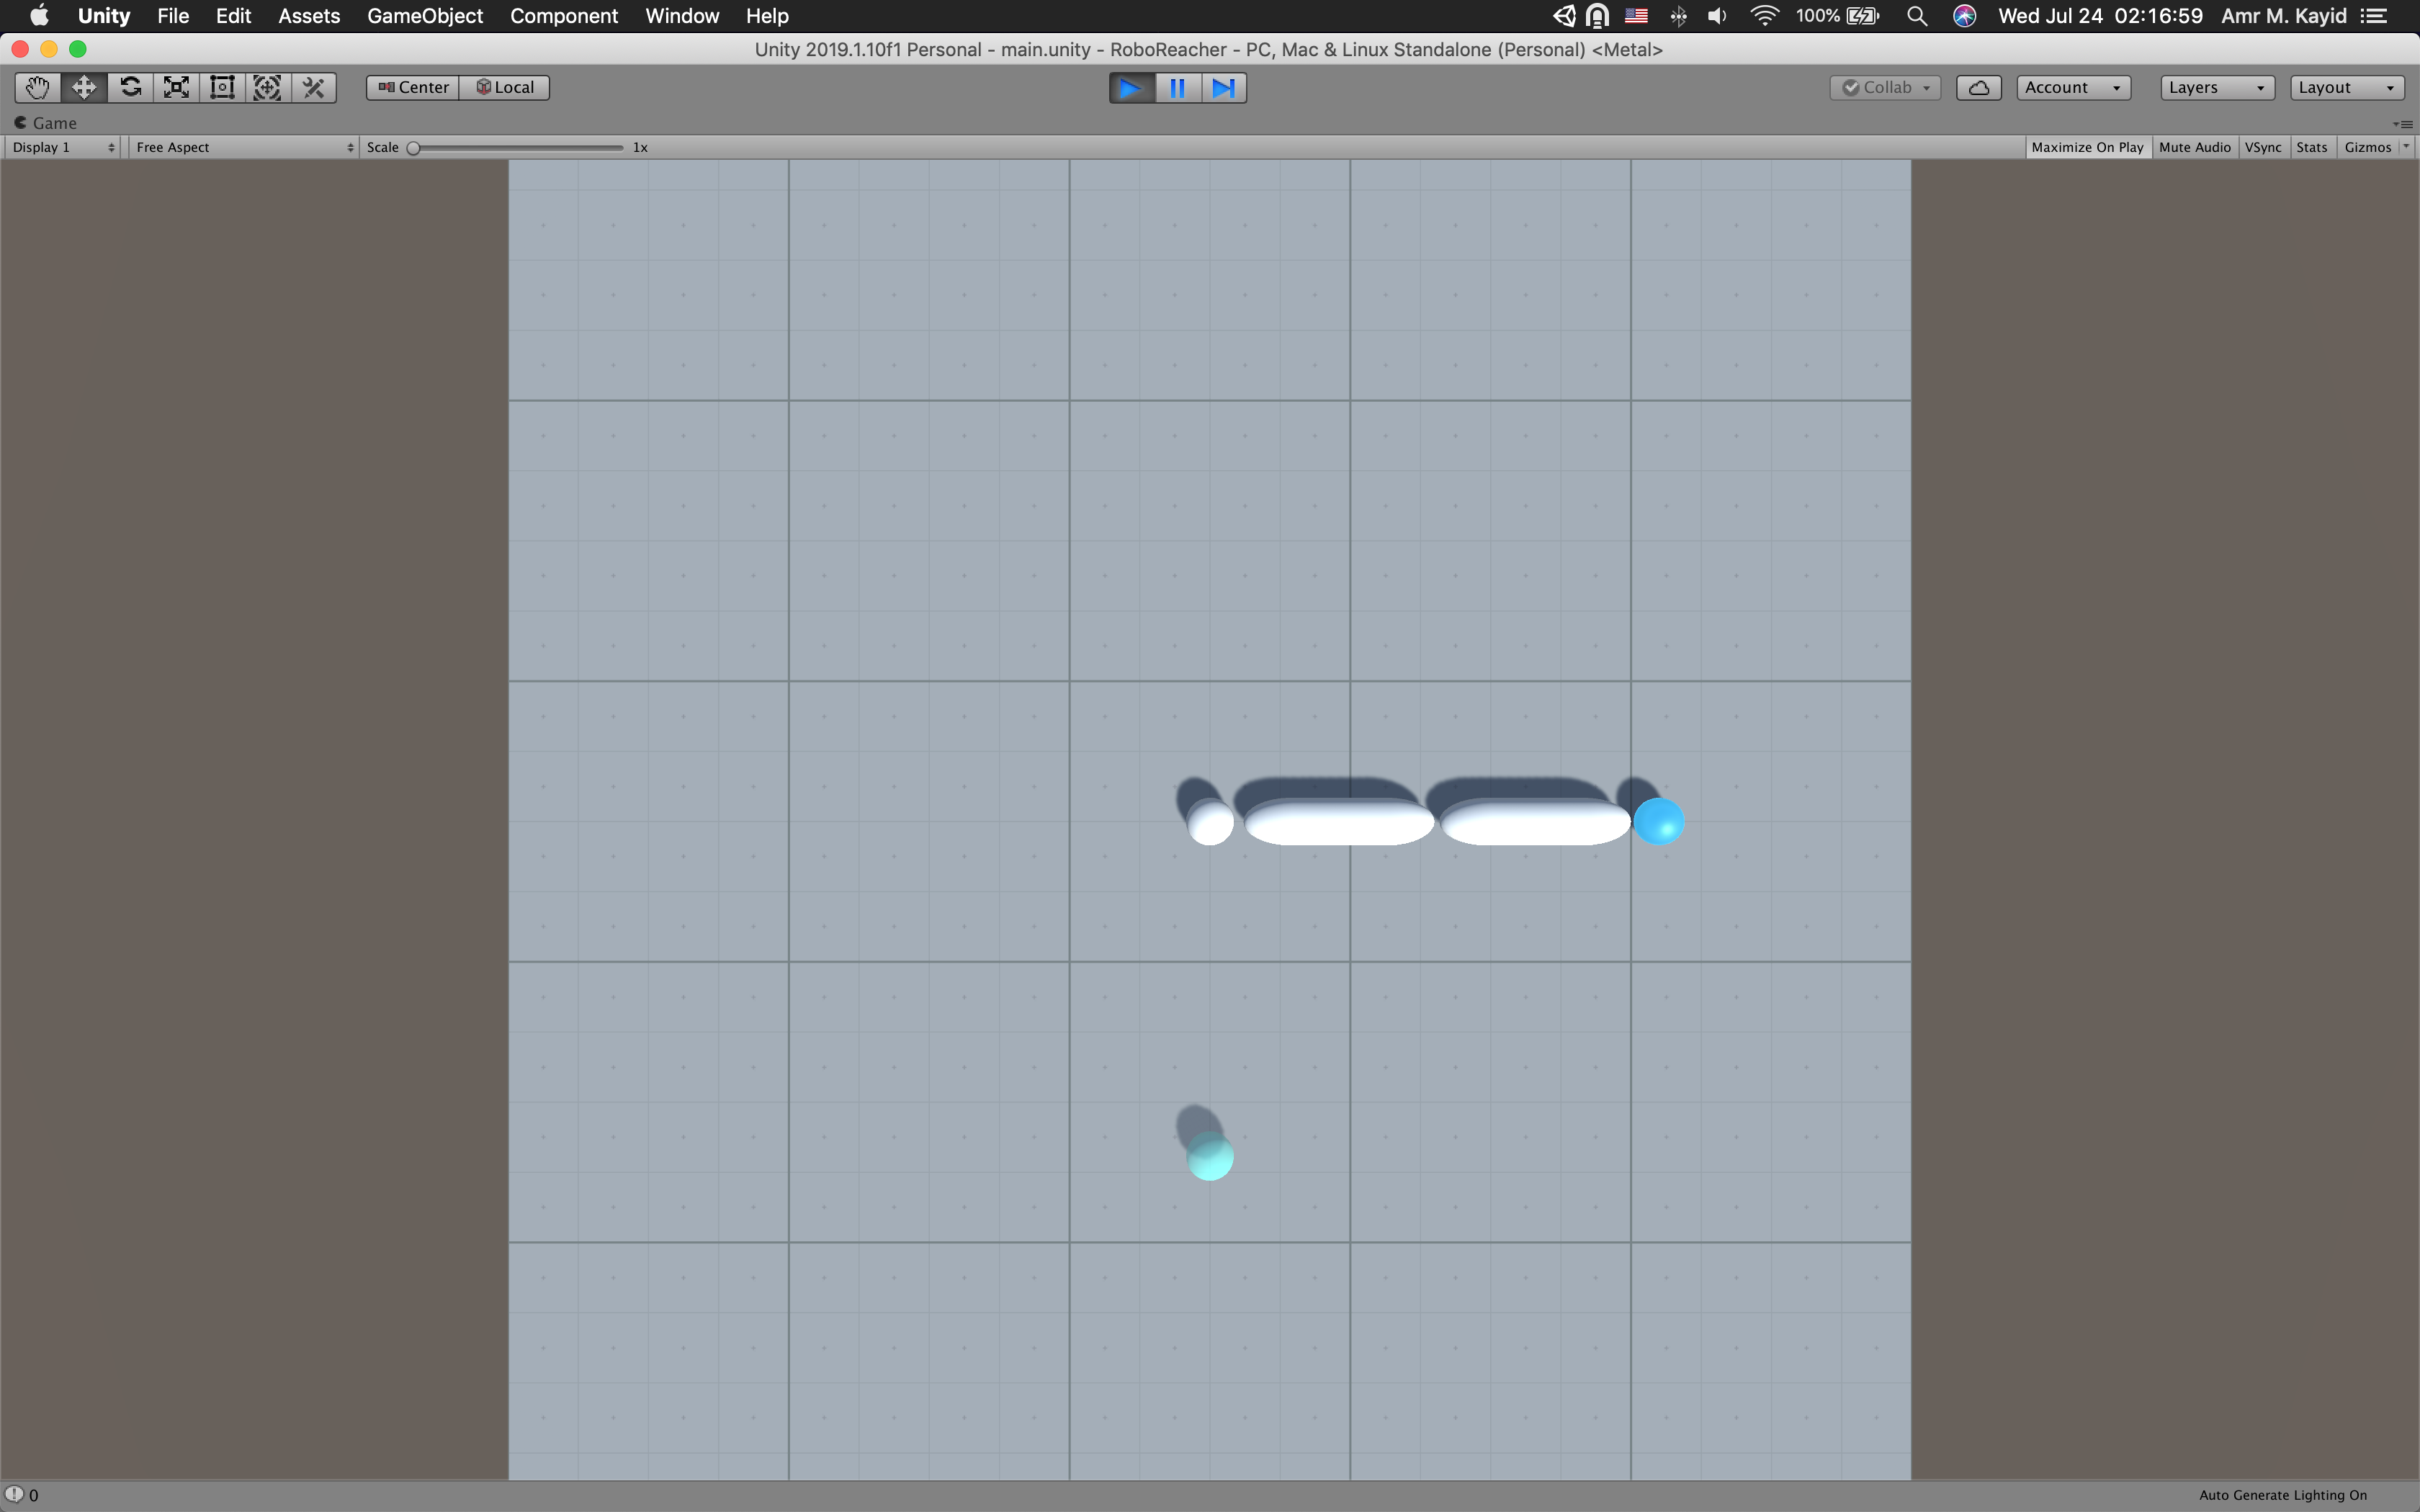
\includegraphics[width=0.7\linewidth]{figures/envs/unity_roboreacher.png}
				\caption{Unity 2-DOF Environment}
				\label{fig:unity_reacher}
\end{figure}

\subsubsection{Reward Function}

The reward function for this environment is different as we modify it to only give a reward of (+0.1) for the agent if the agent can reach the target sphere and keep moving with it along a circular path. Hence, the reward function is described as \textbf{\(R(\tau)=+0.1\)}.

\subsubsection{Experiment Results}

Since this is an evaluation experiment where we have the trained agent from the 3rd experiment, the evaluation will be based on the average reward the agent can obtain after running for 1M time-steps. In this experiment, the agent was able to obtain an average reward ranging from 15 to 20 over the whole testing time-steps as shown in the figure below~\ref{fig:unity2d_avg_reward}.

\begin{figure}[!htb]
		\centering
		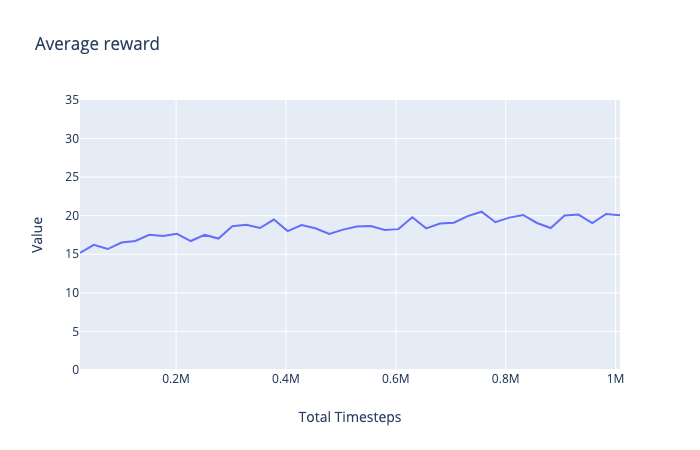
\includegraphics[width=0.7\linewidth]{figures/exps/unity2d.png}
		\caption{Unity 2-DOF Arm Average Reward | Transferring from openai gym engine to unity}
		\label{fig:unity2d_avg_reward}
\end{figure}


\subsubsection{Conclusion}

In this experiment, we were able to transfer learning a pre-trained agent from openai gym environment to a new similar designed unity environment which has a slightly different reward function. We conclude that the agent was able to follow the sphere while it is moving and obtain an average reward of 20. Hence transferring trained agent to new engine was successful.